\documentclass[11pt,a4paper]{article}

\usepackage[margin=2.5cm]{geometry}
\usepackage[T1]{fontenc}
\usepackage{lmodern}
\usepackage{microtype}
\usepackage{amsmath,amssymb,bm}
\usepackage{graphicx}
\usepackage{booktabs,longtable,array}
\usepackage{xcolor}
\usepackage{algorithm}
\usepackage{algpseudocode}
\usepackage[round,authoryear]{natbib}
\usepackage[colorlinks=true,linkcolor=blue!50!black,citecolor=blue!50!black,urlcolor=blue!50!black]{hyperref}
\usepackage[nameinlink,capitalise]{cleveref}

% Numbers in the text come from the code: regenerate with scripts/make_report_assets.py.
% Generated by scripts/make_report_assets.py; do not edit.
\newcommand{\NStocksTotal}{500}
\newcommand{\DataStart}{5 January 2010}
\newcommand{\DataEnd}{30 December 2025}
\newcommand{\SplitDate}{1 January 2019}
\newcommand{\InSampleStart}{4 January 2011}
\newcommand{\InSampleDays}{2011}
\newcommand{\SpecN}{467}
\newcommand{\SpecT}{252}
\newcommand{\MPEdge}{5.58}
\newcommand{\NAboveEdge}{8}
\newcommand{\LamOneShare}{36}
\newcommand{\KeptShare}{60}
\newcommand{\EVMean}{57}
\newcommand{\EVMin}{44}
\newcommand{\EVMax}{71}
\newcommand{\EVMaxDate}{June 2012}
\newcommand{\BaseGrossSR}{1.33}
\newcommand{\BaseNetSR}{\ensuremath{-}1.18}
\newcommand{\BaseGrossRet}{4.5}
\newcommand{\BaseNetRet}{\ensuremath{-}4.0}
\newcommand{\BaseVol}{3.4}
\newcommand{\BaseMaxDD}{\ensuremath{-}33.1}
\newcommand{\BaseTurnover}{0.67}
\newcommand{\BaseStockLegTurnover}{0.34}
\newcommand{\BaseHedgeTurnover}{0.33}
\newcommand{\BaseGrossLev}{1.98}
\newcommand{\BaseOpenMean}{156}
\newcommand{\BaseHolding}{9.0}
\newcommand{\BaseBreakeven}{2.6}
\newcommand{\NVariants}{40}


\newcommand{\todo}[1]{\textcolor{red!70!black}{\textbf{[TODO:} #1\textbf{]}}}
\newcommand{\E}{\mathbb{E}}
\newcommand{\Var}{\operatorname{Var}}
\newcommand{\code}[1]{\texttt{#1}}

\graphicspath{{figures/}}

\title{PCA-Based Statistical Arbitrage on US Equities:\\
\large A Replication of Avellaneda \& Lee (2010) and an Analysis of Its Trading Costs}
\author{Korhan Karadere\\
\small MEng Biomedical Engineering, Imperial College London}
\date{Draft, \today\\ \small\textcolor{red!70!black}{Results are in-sample only; the held-out test period has not been evaluated.}}

\begin{document}
\maketitle

\begin{abstract}
We replicate the PCA-based statistical arbitrage strategy of \citet{avellaneda2010} on the
constituents of the S\&P~500 from 2011 onwards, and test whether it survives realistic costs and
execution. Each day, eigenportfolios of the empirical correlation matrix serve as risk factors, each
stock's residual is modelled as an Ornstein--Uhlenbeck process, and positions are opened when the
residual deviates far from equilibrium. On in-sample data (2011--2018) the original specification
has a gross Sharpe ratio of \BaseGrossSR{}, but at a one-way cost of 5~bps its net Sharpe ratio is
\BaseNetSR{}: it earns only \BaseBreakeven{}~bps per unit of capital traded, and about half of its
trading is hedging. Hedging fewer factors, in line with a random-matrix estimate of how many
eigenvalues exceed noise, and adding a no-trade band raise the break-even cost to about 5.6~bps.
However, trading one day after the signal instead of at the signal's own close removes
\LagLossBest--\LagLossBase\% of the gross Sharpe ratio, and with that realistic timing no rule-based
variant is profitable net of costs. A CNN--Transformer trained directly on the net Sharpe ratio, in
a yearly walk-forward over 2014--2018, trades a seventh as much and loses only \DeepLagLoss\% of its
gross Sharpe ratio to the lag, reaching a break-even cost of \DeepLagBE~bps against
\ALDeepYearsLagBE~bps for the original rule. It still does not clear 5~bps, and about half of its
lagged edge is a systematic long tilt in residuals rather than reversal. The 2019--2025 period is
held out for a single final evaluation (\cref{sec:oos}).
\todo{Finalise the abstract after the held-out test and the multiple-testing correction.}
\end{abstract}

\tableofcontents
\newpage

\section{Introduction}
\label{sec:intro}

Statistical arbitrage covers trading strategies that exploit predictable, short-lived
deviations in the relative prices of securities while holding little exposure to the market
as a whole. The simplest form is pairs trading \citep{gatev2006}: find two stocks that have
historically moved together, and when the spread between them widens, buy the cheap one and
short the expensive one. Generalising from pairs to a whole cross-section requires a model of
what ``moving together'' means for hundreds of stocks at once. A factor model provides one.

\citet{avellaneda2010} (hereafter AL) proposed using principal component analysis (PCA) of the
empirical correlation matrix to extract the factors directly from the data. Each stock's return
is decomposed into a systematic part, explained by a small number of \emph{eigenportfolios},
and an idiosyncratic residual. The cumulative residual is modelled as a mean-reverting
Ornstein--Uhlenbeck (OU) process. When a stock's residual is far below its estimated
equilibrium, the stock is bought and its factor exposure hedged away. Symmetrically, stocks with
residuals far above equilibrium are shorted. The resulting portfolio is close to market- and
factor-neutral, so its profits come from the mean reversion of the residuals.

AL report attractive risk-adjusted returns for US equities over 1997--2007 and note a decline in
performance in the later years of their sample. This project asks three questions:
\begin{enumerate}
  \item Does the PCA residual signal still carry information in the S\&P~500 after 2010?
  \item If it does, is the strategy profitable after realistic trading costs, and if not, where
        do the costs come from?
  \item Which design choices reduce those costs without destroying the signal, and do the
        improvements survive a held-out test period?
\end{enumerate}

\paragraph{Contributions.}
\begin{itemize}
  \item An open, tested implementation of the AL strategy with a pluggable data layer, so the
        same code can run on free data (Yahoo Finance) or survivorship-free data (CRSP).
  \item A decomposition of the strategy's turnover. It shows that the cost of hedging, which is
        incurred mainly when positions open and close, is as large as the cost of trading the
        signal itself.
  \item Evidence that hedging fewer factors, chosen in line with random-matrix theory, and a
        no-trade band roughly double the edge per unit traded.
  \item Evidence that a large part of the measured edge depends on trading at the signal's own
        closing price: a one-day execution lag removes up to half of the gross Sharpe ratio.
  \item A deep-learning signal extractor, trained on the net-of-cost Sharpe ratio in a strict
        walk-forward, that is far more robust to execution lag than the rule-based strategy, and a
        decomposition showing how much of its edge is reversal and how much a systematic tilt.
  \item An evaluation protocol with a strict in-sample/test split enforced by the tooling, and an
        explicit count of every variant tried, so the final results can be corrected for
        multiple testing.
\end{itemize}

\paragraph{Outline.}
\Cref{sec:related} reviews related work. \Cref{sec:data} describes the data,
\cref{sec:method} the methodology, and \cref{sec:impl} the implementation and its validation.
\Cref{sec:protocol} sets out the evaluation protocol, \cref{sec:results} presents results, and
\cref{sec:discussion} discusses them and their limitations.

\section{Related work}
\label{sec:related}

\paragraph{Short-term reversal and pairs trading.}
Short-horizon reversal in individual stock returns is well documented: stocks that performed
poorly over the past week or month tend to outperform in the following period
\citep{lehmann1990,lo1990}. \citet{lo1990} show that a large part of contrarian profits comes
from cross-stock effects and not only from own-stock overreaction. This motivates looking at
returns \emph{relative to} related stocks rather than in isolation. \citet{gatev2006} document
the profitability of a simple distance-based pairs-trading rule over several decades of US data.
\citet{krauss2017} surveys the pairs-trading literature and classifies approaches into distance,
cointegration, time-series, stochastic-control and other methods.

\paragraph{Factor models and PCA.}
Arbitrage pricing theory \citep{ross1976} justifies decomposing returns into exposures to a
small number of pervasive factors plus idiosyncratic noise. \citet{connor1986} show that the
factors can be estimated by principal components when the cross-section is large. How many
factors to keep is a long-standing question. \citet{bai2002} propose information criteria for
it, while random-matrix theory offers a simple benchmark: under the null of pure noise, the
eigenvalues of a sample correlation matrix are confined below the Marchenko--Pastur edge
\citep{marchenko1967}. \citet{laloux1999} and \citet{plerou2002} find that only a small number of
eigenvalues of stock correlation matrices exceed this edge. The rest are statistically
indistinguishable from noise.

\paragraph{PCA statistical arbitrage.}
\citet{avellaneda2010} combine these ingredients: PCA (or sector ETFs) for the factors, an OU
model for the residuals \citep{uhlenbeck1930}, and a threshold rule on a standardised residual,
the \emph{s-score}. They also introduce a volume-adjusted (``trading time'') variant. Their
strategy is the baseline replicated here. \citet{khandani2007} analyse the abrupt losses of
quantitative equity market-neutral funds in August 2007, a reminder that such strategies are
crowded and exposed to sudden deleveraging.
\todo{Add post-2010 replications and extensions, e.g.\ deep-learning variants of residual
mean-reversion trading.}

\paragraph{Trading costs and evaluation.}
With proportional costs, the optimal policy is to leave the portfolio unchanged while it stays
inside a no-trade region \citep{davis1990}. \citet{garleanu2013} show that the optimal portfolio
moves only partially towards its target each period. Both ideas motivate the no-trade band in
\cref{sec:method:costs}. On evaluation, \citet{harvey2016} argue that the large number of
strategies tried by researchers calls for much higher significance thresholds. \citet{bailey2014}
propose the deflated Sharpe ratio, which corrects an observed Sharpe ratio for the number of
trials and for non-normal returns. We count every variant we try for exactly this reason.

\section{Data}
\label{sec:data}

\paragraph{Universe.}
The universe is the current list of S\&P~500 constituents, taken from Wikipedia and saved as a
snapshot file so that every run uses the same list. Of the 503 listed share classes, Yahoo
Finance returns data for \NStocksTotal{}. The three missing are recent spin-offs with no
history in the sample.

\paragraph{Prices and returns.}
Daily closing prices, adjusted for splits and dividends, and daily share volumes are downloaded
from Yahoo Finance for \DataStart{} to \DataEnd{}. The return of stock $i$ on day $t$ is the
simple total return
\begin{equation}
  R_{it} = \frac{P_{it}}{P_{i,t-1}} - 1 .
\end{equation}
Missing prices are \emph{not} filled. A gap leaves a missing return, and the stock cannot be
traded until it has a complete estimation window again (\cref{sec:method}). Yahoo Finance
backfills prices for some companies from before their US listing (e.g.\ SW, FERG, AMCR). These
days carry zero reported volume, so we treat every zero-volume day as a non-trading day.

\paragraph{Survivorship bias.}
Using today's index members for a historical backtest introduces survivorship bias. Stocks that
were removed from the index, acquired or delisted between 2010 and today are missing, and
today's members are by construction companies that survived and mostly grew. For a
market-neutral strategy the direction of the bias is not obvious, since it affects both long and
short legs. It does, however, make the universe less representative and removes exactly the
stocks with the most extreme idiosyncratic moves. All results in this draft should be read with
this caveat. The data layer is built so that the CRSP daily stock file, which provides a
point-in-time universe and delisting returns, can replace Yahoo Finance without changes to the
strategy code (\cref{sec:impl}).
\todo{Re-run on CRSP via WRDS and report the difference.}

\paragraph{Sample split.}
The data are split into an in-sample period, which ends on 31~December~2018, and a held-out test
period from \SplitDate{} to \DataEnd{}. Because the first 252 days are needed to estimate the
model, the first trading day is \InSampleStart{}, giving \InSampleDays{} in-sample trading
days. The split and how it is enforced are described in \cref{sec:protocol}.

\section{Methodology}
\label{sec:method}

The strategy is re-estimated at the close of every trading day $t$ using only returns up to and
including day $t$. \Cref{tab:params} lists the parameters and their baseline values, which
follow AL. \Cref{alg:daily} summarises one day of the procedure.

\begin{table}[ht]
\centering
\caption{Strategy parameters. Baseline values follow \citet{avellaneda2010}.}
\label{tab:params}
\begin{tabular}{llr}
\toprule
Symbol & Meaning & Baseline \\
\midrule
$M$ & correlation estimation window (days) & 252 \\
$m$ & number of eigenportfolios (factors) & 15 \\
$L$ & residual estimation window (days) & 60 \\
$\kappa_{\min}$ & minimum mean-reversion speed (per year) & $252/30 \approx 8.4$ \\
$\bar s_{\text{open}}$ & entry threshold & 1.25 \\
$\bar s_{\text{cl}}$ & exit threshold, longs & 0.50 \\
$\bar s_{\text{cs}}$ & exit threshold, shorts & 0.75 \\
$q$ & notional per position (fraction of capital) & 0.01 \\
$c$ & one-way transaction cost & 5~bps \\
$\delta$ & no-trade band (fraction of capital) & 0 (off) \\
\bottomrule
\end{tabular}
\end{table}

\subsection{Eigenportfolios}
\label{sec:method:pca}

Let $\mathcal U_t$ be the set of $N_t$ stocks with a complete return history over the window
$\{t-M+1,\dots,t\}$. For each such stock compute the sample mean $\bar R_i$ and standard
deviation $\sigma_i$ over the window, and the standardised returns
$Y_{is} = (R_{is} - \bar R_i)/\sigma_i$. The empirical correlation matrix is
\begin{equation}
  \rho_{ij} = \frac{1}{M-1} \sum_{s=t-M+1}^{t} Y_{is} Y_{js} .
\end{equation}
Let $\lambda_1 \ge \lambda_2 \ge \dots \ge \lambda_{N_t}$ be its eigenvalues and
$\bm v^{(1)},\dots,\bm v^{(N_t)}$ the corresponding unit eigenvectors. The first $m$
eigenvectors define the \emph{eigenportfolios}, with dollar weights
\begin{equation}
  Q_i^{(j)} = \frac{v_i^{(j)}}{\sigma_i}, \qquad j = 1,\dots,m,
  \label{eq:eigenportfolio}
\end{equation}
and returns $F_{js} = \sum_i Q_i^{(j)} R_{is}$. Dividing by $\sigma_i$ maps the eigenvector,
which lives in the space of standardised returns, back to dollar holdings, so volatile stocks
receive smaller weights. Eigenvectors are only defined up to sign. We choose the sign that
makes $\sum_i v_i^{(j)} > 0$. This does not affect the strategy but makes the first factor read
as a long-only ``market'' portfolio.

\subsection{Factor regression}
\label{sec:method:regression}

For each stock $i \in \mathcal U_t$, the last $L$ daily returns are regressed on the
contemporaneous eigenportfolio returns:
\begin{equation}
  R_{is} = \alpha_i + \sum_{j=1}^{m} \beta_{ij} F_{js} + \varepsilon_{is},
  \qquad s = t-L+1,\dots,t .
  \label{eq:regression}
\end{equation}
The correlation matrix uses a long window ($M=252$) because the factors need many observations
to be estimated stably. The regression uses a short window ($L=60$) because factor loadings
drift over time. All $N_t$ regressions share the same design matrix, so they are solved with a
single least-squares call (\cref{sec:impl}).

\subsection{Residual process}
\label{sec:method:ou}

The cumulative residual
\begin{equation}
  X_{ik} = \sum_{s=t-L+1}^{t-L+k} \varepsilon_{is}, \qquad k = 1,\dots,L,
\end{equation}
measures how far stock $i$ has drifted from the path implied by its factor exposures. Following
AL, it is modelled as an Ornstein--Uhlenbeck process,
\begin{equation}
  dX_i = \kappa_i (m_i - X_i)\, dt + \sigma_i^{\text{OU}}\, dW_i ,
  \label{eq:ou}
\end{equation}
which reverts to the level $m_i$ at speed $\kappa_i$. Sampled daily, \cref{eq:ou} is exactly an
AR(1) process (\cref{app:ou}),
\begin{equation}
  X_{i,k+1} = a_i + b_i X_{ik} + \zeta_{i,k+1},
  \label{eq:ar1}
\end{equation}
which is fitted by least squares. The OU parameters follow as
\begin{equation}
  \kappa_i = -252 \ln b_i, \qquad
  m_i = \frac{a_i}{1-b_i}, \qquad
  \sigma_{\text{eq},i} = \sqrt{\frac{\Var(\zeta_i)}{1-b_i^2}},
  \label{eq:ou-params}
\end{equation}
where $\sigma_{\text{eq},i}$ is the standard deviation of the stationary distribution of
$X_i$. If $b_i \notin (0,1)$, the fitted process is not mean-reverting and the stock is not
eligible on that day. The stock is also ineligible if its estimated mean-reversion time
$1/\kappa_i$ exceeds $1/\kappa_{\min}$, about 30 trading days, i.e.\ half the estimation window.
Reversion slower than that cannot be estimated reliably from $L=60$ observations.

\subsection{The s-score}
\label{sec:method:sscore}

For eligible stocks, the \emph{s-score} is the distance of the current cumulative residual from
its equilibrium, measured in equilibrium standard deviations:
\begin{equation}
  s_i = \frac{X_{iL} - \tilde m_i}{\sigma_{\text{eq},i}}, \qquad
  \tilde m_i = m_i - \frac{1}{|\mathcal E_t|}\sum_{k \in \mathcal E_t} m_k ,
  \label{eq:sscore}
\end{equation}
where $\mathcal E_t$ is the set of eligible stocks. Centring the equilibrium levels across
stocks removes a common bias in the estimated $m_i$ that AL attribute to the regression
intercepts. Because \cref{eq:regression} includes an intercept, the residuals sum to zero over
the window, so $X_{iL} = 0$ exactly and $s_i = -\tilde m_i/\sigma_{\text{eq},i}$. A strongly
negative s-score means the stock is cheap relative to its factors and is expected to rise
relative to them. A strongly positive s-score means the reverse.

\subsection{Trading rule}
\label{sec:method:rule}

Each stock is in one of three states: long ($+1$), flat ($0$) or short ($-1$). States are
updated daily by the rule in \cref{tab:rule}. Exits are applied before entries, so a position can
reverse on a single day. The gap between the entry and exit thresholds (hysteresis) prevents
positions from being repeatedly opened and closed as the s-score fluctuates around a single
threshold.

\begin{table}[ht]
\centering
\caption{Trading rule on the s-score.}
\label{tab:rule}
\begin{tabular}{lll}
\toprule
Current state & Condition & New state \\
\midrule
flat & $s_i < -\bar s_{\text{open}}$ & long \\
flat & $s_i > +\bar s_{\text{open}}$ & short \\
long & $s_i > -\bar s_{\text{cl}}$ & flat \\
short & $s_i < +\bar s_{\text{cs}}$ & flat \\
any & stock ineligible on day $t$ & flat \\
\bottomrule
\end{tabular}
\end{table}

\subsection{Portfolio construction and hedging}
\label{sec:method:portfolio}

Let $\theta_{it} \in \{-1,0,1\}$ be the state of stock $i$ and $w_i = q\,\theta_{it}$ the
dollar position in the stock. To isolate the residual, each position is hedged by selling
$\beta_{ij} w_i$ dollars' worth of eigenportfolio $j$ for every $j$. One unit of eigenportfolio
$j$ holds $Q_k^{(j)}$ dollars of stock $k$, so the hedges can be netted back into single-stock
holdings. Writing $Q \in \mathbb R^{N\times m}$ and $B \in \mathbb R^{N\times m}$ for the
matrices of eigenportfolio weights and betas, the net holdings are
\begin{equation}
  \bm w^{\text{net}} = \bm w - Q B^\top \bm w .
  \label{eq:netting}
\end{equation}
Within the estimation window the portfolio return is
$\sum_k w^{\text{net}}_k R_k = \sum_i w_i (R_i - \sum_j \beta_{ij} F_j) = \sum_i w_i(\alpha_i + \varepsilon_i)$:
the factor exposures cancel by construction and only the residuals remain.

\paragraph{Daily versus frozen hedges.}
In AL's specification, \cref{eq:netting} is re-evaluated every day with that day's $Q$ and $B$,
so the hedge of every open position is continuously updated. We also implement a
\emph{frozen} hedge. The stock-space hedge of position $i$,
$\bm h_i = -w_i\, Q^{(\tau_i)} \bm\beta_i^{(\tau_i)}$, is computed once on the entry day
$\tau_i$ and held unchanged until the position is closed. Net holdings are then
$\bm w + \sum_i \bm h_i$. The trading signals are identical in both modes. Only the hedge
differs.

\subsection{Cost-reduction mechanisms}
\label{sec:method:costs}

\paragraph{Volume-adjusted returns.}
AL's ``trading time'' variant replaces $R_{is}$ in \cref{eq:regression} by
$R_{is}\,\langle V_i\rangle_s / V_{is}$, where $V_{is}$ is the share volume and
$\langle V_i\rangle_s$ its trailing 10-day mean ending on day $s$. Returns on heavy-volume days,
which are more likely to reflect news, are shrunk, and returns on light-volume days are
amplified. Only the signal uses adjusted returns. The factors and the P\&L use actual returns.

\paragraph{No-trade band.}
Given the target holdings $w^\ast_{kt}$ from \cref{eq:netting} and yesterday's holdings
$w_{k,t-1}$, each stock is traded only if its required adjustment exceeds the band $\delta$:
\begin{equation}
  w_{kt} =
  \begin{cases}
    w^\ast_{kt} & \text{if } |w^\ast_{kt} - w_{k,t-1}| > \delta, \\
    w_{k,t-1} & \text{otherwise.}
  \end{cases}
  \label{eq:band}
\end{equation}
This is a simple form of the no-trade region that is optimal under proportional costs
\citep{davis1990}. It removes the many small hedge adjustments spread across all stocks, at the
price of a small tracking error to the target.

\paragraph{Fewer factors.}
Every eigenportfolio holds a position in every stock. So each factor hedged adds a basket trade
across the entire universe whenever a position is opened or closed. Hedging fewer factors
reduces this cost but leaves more systematic risk in the residual. This trade-off is studied
in \cref{sec:results:factors}.

\subsection{Backtest accounting}
\label{sec:method:accounting}

Holdings determined at the close of day $t$ earn the returns of day $t+1$, so no information from
day $t+1$ is used to form them. Capital is fixed at one unit, without compounding, as in AL.
Daily P\&L, as a fraction of capital, is
\begin{align}
  \text{gross}_{t+1} &= \sum_k w_{kt}\, R_{k,t+1}, \\
  \text{cost}_{t+1} &= c \sum_k \left| w_{kt} - w_{k,t-1} \right|, \\
  \text{net}_{t+1} &= \text{gross}_{t+1} - \text{cost}_{t+1}.
\end{align}
The quantity $\text{TO}_t = \sum_k |w_{kt} - w_{k,t-1}|$ is the daily one-way turnover. A missing
next-day return of a held stock (for example after a delisting) is treated as zero.

Annualised return and volatility are $252$ times the mean and $\sqrt{252}$ times the standard
deviation of daily net P\&L, and the Sharpe ratio is their ratio. Because the strategy is
market-neutral and self-financing apart from margin, no risk-free rate is subtracted. We also
report the \emph{break-even cost}
\begin{equation}
  c^\ast = \frac{\overline{\text{gross}}}{\overline{\text{TO}}},
  \label{eq:breakeven}
\end{equation}
the one-way cost at which net P\&L would be zero. It measures the gross edge per unit of capital
traded and is the most direct summary of whether a variant can survive costs.

\begin{algorithm}[ht]
\caption{One trading day $t$ of the strategy}
\label{alg:daily}
\begin{algorithmic}[1]
\State $\mathcal U_t \gets$ stocks with complete returns over $[t-M+1, t]$
\State $Q \gets$ eigenportfolio weights from the top $m$ eigenvectors of $\rho$ \Comment{\cref{eq:eigenportfolio}}
\State $F \gets R_{[t-L+1,t],\,\mathcal U_t}\, Q$ \Comment{factor returns, $L\times m$}
\State $(\bm\alpha, B, \bm\varepsilon) \gets$ least squares of $R$ on $[\bm 1, F]$ \Comment{\cref{eq:regression}}
\State $X \gets \operatorname{cumsum}(\bm\varepsilon)$; fit AR(1); compute $\kappa, m, \sigma_{\text{eq}}$ \Comment{\cref{eq:ar1,eq:ou-params}}
\State $\bm s \gets$ s-scores, NaN where $\kappa < \kappa_{\min}$ \Comment{\cref{eq:sscore}}
\State $\bm\theta_t \gets$ update states with the rule of \cref{tab:rule}
\State $\bm w^\ast \gets q\bm\theta_t - Q B^\top q\bm\theta_t$ \Comment{or frozen hedges}
\State $\bm w_t \gets$ apply the no-trade band to $\bm w^\ast$ \Comment{\cref{eq:band}}
\State earn $\bm w_t^\top R_{t+1}$; pay $c\,\|\bm w_t - \bm w_{t-1}\|_1$
\end{algorithmic}
\end{algorithm}

\section{Implementation and validation}
\label{sec:impl}

\subsection{Software design}

The strategy is implemented as a Python package (\code{pca\_stat\_arb}) built on NumPy and
pandas. \Cref{tab:modules} lists its modules. Three design decisions matter for the
correctness and extensibility of the results.

\begin{enumerate}
  \item \textbf{A single data contract.} Every data source implements one interface,
        \code{ReturnsSource}, whose output is a table of daily total returns indexed by date and
        security. Nothing downstream depends on where the data came from, so replacing Yahoo
        Finance with CRSP requires only a new loader.
  \item \textbf{Configuration as data.} All parameters live in typed, immutable configuration
        objects loaded from YAML files and are checked for validity when loaded. Each experiment
        is a named set of overrides of the baseline configuration, so every reported variant can
        be reproduced from a file.
  \item \textbf{Vectorised daily step.} Within each day all computations run on whole arrays
        rather than looping over stocks: one symmetric eigendecomposition, one multi-target
        least-squares solve for all regressions in \cref{eq:regression}, and closed-form AR(1)
        estimates for all stocks at once. A full backtest over 15 years and 500 stocks takes
        about 45 seconds on a laptop, which makes systematic parameter sweeps practical.
\end{enumerate}

\begin{table}[ht]
\centering
\caption{Package structure.}
\label{tab:modules}
\small
\begin{tabular}{@{}l>{\raggedright\arraybackslash}p{0.52\textwidth}@{}}
\toprule
Module & Responsibility \\
\midrule
\code{config} & typed configuration, validation \\
\code{data.base}, \code{data.yfinance\_source} & data interface; Yahoo Finance loader with caching and cleaning \\
\code{data.universe} & constituent list snapshot \\
\code{pca} & eigenportfolios (\cref{sec:method:pca}) \\
\code{residuals} & factor regression, OU fit, s-scores (\cref{sec:method:regression,sec:method:ou,sec:method:sscore}) \\
\code{signals} & trading rule (\cref{sec:method:rule}) \\
\code{backtest} & daily loop, hedging, costs (\cref{sec:method:portfolio,sec:method:costs,sec:method:accounting}) \\
\code{metrics} & performance statistics, in-sample/test split \\
\code{scripts/experiments.py} & parallel variant runner, in-sample by default \\
\code{scripts/make\_report\_assets.py} & all figures, tables and numbers in this report \\
\bottomrule
\end{tabular}
\end{table}

\paragraph{Reproducibility of this report.}
Every figure, results table and quoted statistic in this report is produced by
\code{scripts/make\_report\_assets.py} directly from the code's output. The numbers in the text are
inserted as generated \LaTeX{} macros rather than typed by hand, so the report cannot drift out
of sync with the code. The script truncates the data at the split date before doing anything
else, so no held-out data can enter the report until the final evaluation.

\subsection{Validation on synthetic data}
\label{sec:impl:tests}

Backtests can fail silently: a subtle bug can produce plausible-looking but wrong P\&L. The
implementation is therefore tested on a simulated market where the true structure is known.
Returns are generated from three factors (a dominant market factor and two zero-mean
``sector'' factors) plus idiosyncratic residuals whose cumulative sums follow an OU process with
known $\kappa$. \Cref{tab:tests} summarises the automated tests, all of which pass.

\begin{table}[ht]
\centering
\caption{Automated tests. All run on synthetic data with known structure.}
\label{tab:tests}
\begin{tabular}{p{0.38\textwidth}p{0.54\textwidth}}
\toprule
Test & Property checked \\
\midrule
Spectrum vs.\ Marchenko--Pastur edge & exactly the 3 true factors have eigenvalues above $(1+\sqrt{N/T})^2$; the first eigenvector is the market \\
Orthogonality & regression residuals are orthogonal to the factors, and $X_{iL}=0$ \\
OU recovery & the AR(1) mapping recovers the true $\kappa$ (up to known small-sample bias) \\
s-score eligibility & slow or non-mean-reverting residuals yield no s-score \\
Trading rule & every transition in \cref{tab:rule}, including same-day reversal \\
\textbf{No look-ahead} (three variants) & replacing all data after day $t$ with random noise leaves every holding up to day $t$ unchanged, for daily hedges, frozen hedges with volume adjustment, and the no-trade band \\
End-to-end profitability & the strategy is profitable on the synthetic mean-reverting market \\
Hedge modes & frozen hedges give identical signals with lower turnover, and are released on exit \\
No-trade band & every executed trade exceeds $\delta$; turnover falls \\
Costs & costs reduce net P\&L and leave gross P\&L unchanged \\
Missing data & a stock with a data gap is not traded until it has a full window again \\
\bottomrule
\end{tabular}
\end{table}

The look-ahead tests are the most important. Look-ahead bias, the use of information that would
not have been available at the time of the trade, is the most common way a backtest overstates
performance. Rather than relying on a careful reading of the code, these tests check the
property mechanically for every hedging mode.

\paragraph{Consistency checks on real data.}
On the real data we additionally verified that the recorded states never violate the trading
rule. Across all stocks and in-sample days, no flat stock with $|s_i| > \bar s_{\text{open}}$
failed to open the corresponding position.

\section{Evaluation protocol}
\label{sec:protocol}

Backtested strategies are routinely overfitted. When many variants are tried on the same data,
the best one looks good partly by luck \citep{harvey2016,bailey2014}. We therefore fixed the
following protocol before running any experiment.

\begin{enumerate}
  \item \textbf{Split.} Data before \SplitDate{} are in-sample and used for all design and
        parameter choices. Data from \SplitDate{} to \DataEnd{} are the held-out test.
  \item \textbf{Enforcement by tooling.} The experiment runner reports in-sample statistics only.
        Test-period statistics appear only when the flag \code{--reveal-test} is passed, which will
        happen once, for a small set of final variants chosen in advance. The report-generation
        script cuts the data at the split date before it does anything else.
  \item \textbf{Trial counting.} Every variant run is saved with its configuration. At the time of
        writing, \NVariants{} distinct variants have been evaluated in-sample
        (\cref{app:variants}). This count will enter the deflated Sharpe ratio of the final
        results.
  \item \textbf{Fixed costs.} All variants are compared at the same one-way cost of 5~bps, the
        value used by AL. The break-even cost $c^\ast$ (\cref{eq:breakeven}) shows how sensitive
        each conclusion is to that assumption.
\end{enumerate}

\todo{Add the deflated Sharpe ratio, block-bootstrap confidence intervals for the Sharpe ratio,
and cost-sensitivity curves.}

\section{Results}
\label{sec:results}

All results in \cref{sec:results:factors-structure,sec:results:baseline,sec:results:variants,sec:results:factors,sec:results:band}
are in-sample (\InSampleStart{} to 31~December~2018). \Cref{tab:main} summarises the main
variants. \Cref{app:variants} lists all \NVariants{} variants evaluated.

\begin{table}[ht]
\centering
\caption{In-sample performance of selected variants at 5~bps one-way cost. SR: annualised
Sharpe ratio. Net return: annualised, as a fraction of capital. Max DD: maximum drawdown of
cumulative net P\&L. Turnover: mean daily one-way turnover in units of capital. BE: break-even
one-way cost (\cref{eq:breakeven}).}
\label{tab:main}
\small
\setlength{\tabcolsep}{4pt}
\begin{tabular}{@{}lrrrrrr@{}}
\toprule
Variant & Gross SR & Net SR & Net return & Max DD & Turnover & BE (bps)\\
\midrule
AL baseline ($m=15$, daily hedge) & 1.33 & \ensuremath{-}1.18 & \ensuremath{-}4.0\% & \ensuremath{-}33.1\% & 0.67 & 2.6\\
Frozen hedge & 1.16 & \ensuremath{-}1.10 & \ensuremath{-}3.7\% & \ensuremath{-}31.6\% & 0.61 & 2.6\\
Volume-adjusted signal & 1.29 & \ensuremath{-}1.15 & \ensuremath{-}3.8\% & \ensuremath{-}30.4\% & 0.63 & 2.6\\
Wider entry ($\bar s_{\text{open}}=2.0$) & 0.83 & \ensuremath{-}1.14 & \ensuremath{-}2.1\% & \ensuremath{-}17.0\% & 0.28 & 2.1\\
$m=3$ & 1.29 & 0.09 & 0.4\% & \ensuremath{-}9.1\% & 0.41 & 5.4\\
$m=3$, band $0.0005$ & 1.24 & 0.17 & 0.7\% & \ensuremath{-}7.6\% & 0.36 & 5.8\\
$m=8$, band $0.002$ & 1.44 & 0.15 & 0.6\% & \ensuremath{-}7.5\% & 0.37 & 5.6\\
\bottomrule
\end{tabular}

\end{table}

\subsection{Factor structure}
\label{sec:results:factors-structure}

\Cref{fig:spectrum} shows the eigenvalue spectrum of the correlation matrix of \SpecN{} stocks
over the 252 days ending on the last in-sample day. The largest eigenvalue alone accounts for
\LamOneShare\% of total variance, and the 15 kept factors for \KeptShare\%. Only \NAboveEdge{}
eigenvalues exceed the Marchenko--Pastur edge of \MPEdge{}, the upper limit of the eigenvalue
distribution expected if returns were uncorrelated noise. So by this criterion, roughly half of
AL's 15 factors cannot be distinguished from noise at this date.

\begin{figure}[ht]
\centering
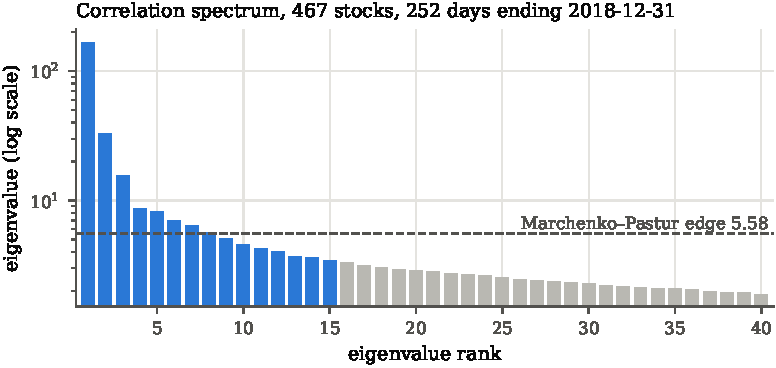
\includegraphics[width=\textwidth]{spectrum}
\caption{Leading 40 eigenvalues of the 252-day correlation matrix ending 31~December~2018 (log
scale). Blue bars are the 15 factors kept in the baseline. The dashed line is the
Marchenko--Pastur edge $(1+\sqrt{N/T})^2$ for $N=\SpecN$, $T=\SpecT$.}
\label{fig:spectrum}
\end{figure}

The leading eigenvectors have clear economic interpretations (\cref{fig:sectors}). The first
loads positively on every sector: it is the market. The second contrasts defensive,
interest-rate-sensitive sectors (utilities, real estate, consumer staples) with the rest of the
market. The third separates information technology from financials and energy, a growth-versus-value
pattern. The factors are therefore recognisable risk factors, even though PCA was not told
anything about sectors.

\begin{figure}[ht]
\centering
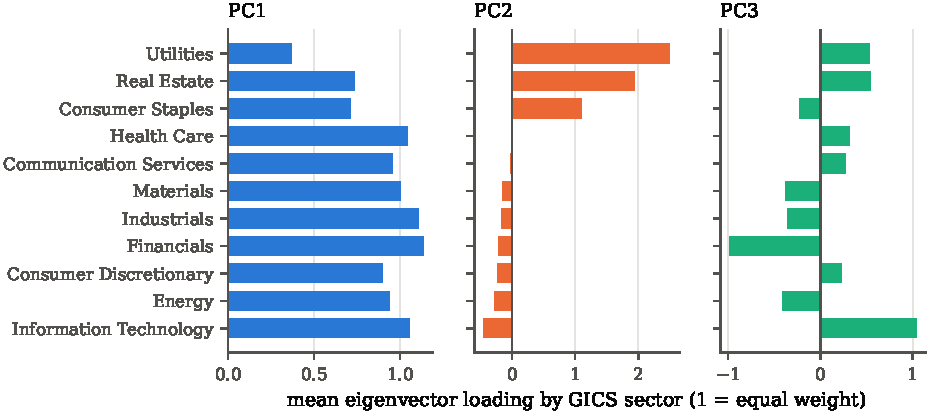
\includegraphics[width=\textwidth]{sector_loadings}
\caption{Mean eigenvector loading of the first three principal components by GICS sector, for the
same window as \cref{fig:spectrum}. Loadings are scaled by $\sqrt N$, so a value of 1 corresponds
to an equal-weighted portfolio.}
\label{fig:sectors}
\end{figure}

The share of variance explained by the 15 factors varies considerably over time
(\cref{fig:explained}). It averages \EVMean\% and ranges from \EVMin\% to \EVMax\%, peaking in
\EVMaxDate{}, when the trailing window covers the August 2011 sell-off and the European
sovereign debt crisis, a period of unusually high correlation across stocks. The amount of risk that is ``systematic'' is therefore itself time-varying, which argues
for choosing $m$ adaptively rather than fixing it.

\begin{figure}[ht]
\centering
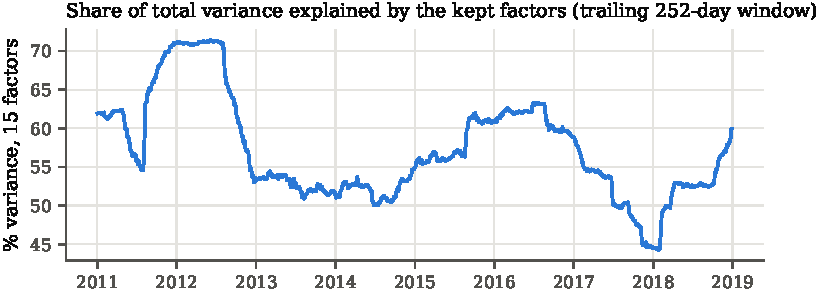
\includegraphics[width=\textwidth]{explained_variance}
\caption{Share of total variance explained by the 15 leading eigenvalues, using a trailing
252-day window.}
\label{fig:explained}
\end{figure}

\subsection{Baseline replication}
\label{sec:results:baseline}

\Cref{fig:sscore} illustrates the trading rule for one stock. The s-score of JPMorgan Chase
fluctuates within roughly $\pm 2$, and positions are opened when it crosses $\pm 1.25$ and closed
as it reverts. Across the in-sample period an average of \BaseOpenMean{} positions are open, and a
position is held for about \BaseHolding{} trading days.

\begin{figure}[ht]
\centering
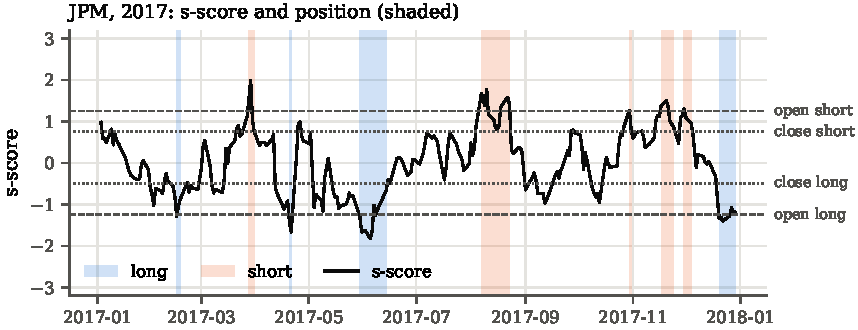
\includegraphics[width=\textwidth]{sscore_example}
\caption{s-score of JPMorgan Chase (JPM) in 2017 under the baseline specification, with entry
(dashed) and exit (dotted) thresholds. Shaded regions mark open long (blue) and short (orange)
positions.}
\label{fig:sscore}
\end{figure}

The baseline earns a gross annualised return of \BaseGrossRet\% with a volatility of
\BaseVol\%, i.e.\ a gross Sharpe ratio of \BaseGrossSR{} (\cref{fig:cumpnl}). The residual
mean-reversion signal is therefore still present in the S\&P~500 after 2010. After 5~bps
one-way costs, however, the annualised return is \BaseNetRet\% and the net Sharpe ratio
\BaseNetSR{}. The strategy trades \BaseTurnover{} times its capital per day, so it pays roughly
$0.67 \times 252 \times 5\,\text{bps} \approx 8.4\%$ a year in costs, about twice its gross
return. Equivalently, its gross edge is only \BaseBreakeven{}~bps per unit traded, half of the
assumed cost.

\begin{figure}[ht]
\centering
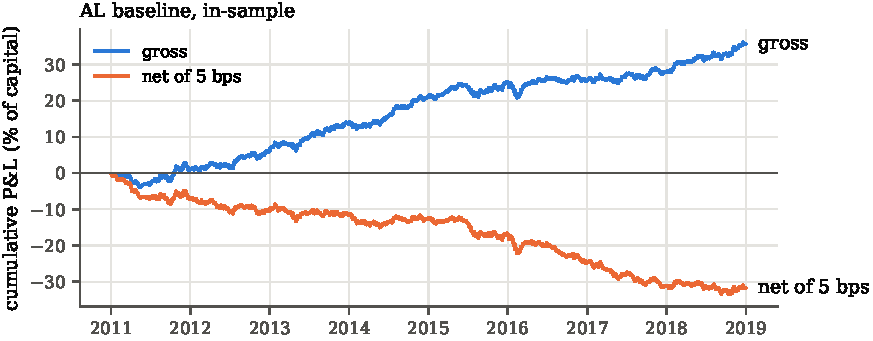
\includegraphics[width=\textwidth]{cum_pnl_baseline}
\caption{Cumulative in-sample P\&L of the baseline, gross and net of 5~bps one-way costs, as a
percentage of (fixed) capital.}
\label{fig:cumpnl}
\end{figure}

\paragraph{Where the turnover comes from.}
Of the \BaseTurnover{} daily turnover, \BaseStockLegTurnover{} is the stock leg, i.e.\ opening and
closing the positions themselves. The remaining \BaseHedgeTurnover{} is hedge trading. Hedging
therefore doubles the strategy's trading costs. As the next subsection shows, most of the hedge
turnover is \emph{not} the daily re-hedging of existing positions but the hedge baskets traded
when positions open and close.

\subsection{Hedge mode, volume adjustment and thresholds}
\label{sec:results:variants}

\paragraph{Frozen hedges} reduce turnover only from 0.67 to 0.61, and they lower the gross Sharpe
ratio from 1.33 to 1.16 because the hedges go stale. Daily re-hedging is therefore cheap: about
0.06 of turnover per day. The large hedge cost comes from building and unwinding the hedge
baskets, which frozen hedging does not change.

\paragraph{The volume-adjusted signal} leaves the break-even cost unchanged at 2.6~bps and
slightly lowers the gross Sharpe ratio (1.29). Combined with frozen hedges it performs worse
still (gross Sharpe 1.01). This contrasts with AL, who found that trading time improved
performance in 2003--2007.

\paragraph{Wider entry thresholds} cut turnover substantially, from 0.67 at
$\bar s_{\text{open}} = 1.25$ to 0.28 at $2.0$, but lower gross returns in proportion or more:
the break-even cost falls from 2.6 to 2.1~bps. Larger deviations are thus \emph{not} more
profitable per unit traded. Exiting later (at $s=0$ or beyond) does not help either. Changing the
residual window to 90 days or the $\kappa_{\min}$ filter also leaves the break-even cost at or
below the baseline (\cref{app:variants}).

\subsection{Number of factors}
\label{sec:results:factors}

The number of hedged factors is the most important design choice (\cref{fig:tradeoff}). The
gross Sharpe ratio rises from 0.74 with a single (market) factor to a maximum of 1.55 at
$m=8$, then falls to 1.33 at $m=15$ and 1.16 at $m=30$. Turnover rises steadily with $m$, from
0.36 to 1.09, because every additional factor adds a basket trade across the whole universe
whenever a position is opened or closed. The break-even cost is about 5~bps for $m \le 3$ and
declines for larger $m$, to 2.6~bps at AL's $m=15$ and 1.4~bps at $m=30$.

Two observations stand out. First, the gross Sharpe ratio peaks at $m=8$, the same number of
eigenvalues that exceed the Marchenko--Pastur edge in \cref{fig:spectrum}. Factors beyond the
noise edge seem to add estimation noise to the residuals rather than remove systematic risk.
Second, a few factors suffice to remove most of the systematic risk at a fraction of the hedging
cost.

\begin{figure}[ht]
\centering
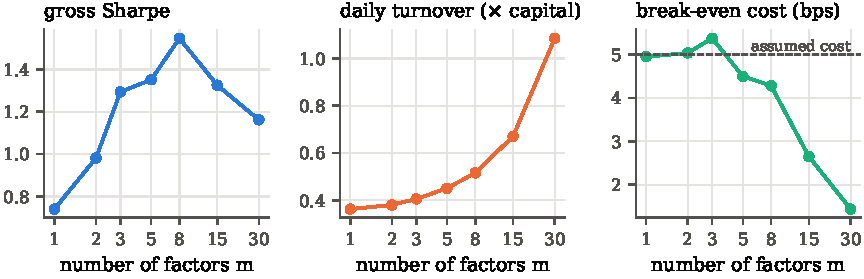
\includegraphics[width=\textwidth]{factor_tradeoff}
\caption{Gross Sharpe ratio, mean daily turnover and break-even cost as a function of the number
of hedged factors $m$ (log scale), in-sample. All other parameters at baseline values. The
dashed line marks the assumed cost of 5~bps.}
\label{fig:tradeoff}
\end{figure}

\subsection{No-trade band}
\label{sec:results:band}

The no-trade band reduces turnover for every number of factors at a small cost in gross Sharpe
ratio (\cref{tab:main} and \cref{app:variants}). With $m=15$, a band of $\delta = 0.002$ cuts
turnover from 0.67 to 0.49 and raises the break-even cost from 2.6 to 3.5~bps, which is still not
enough. Combined with fewer factors, the best in-sample variants reach break-even costs of
5.6--5.8~bps and net Sharpe ratios of about 0.15. Examples are $m=8$ with $\delta=0.002$ (gross
Sharpe 1.44) and $m=3$ with $\delta = 0.0005$ (gross Sharpe 1.24). These are modest numbers. After
correcting for the \NVariants{} variants tried, they are unlikely to be statistically
distinguishable from zero.

\subsection{Held-out test}
\label{sec:oos}

\todo{Pre-register the final variants (proposed: AL baseline; $m=8$ with $\delta=0.002$; $m=3$
with $\delta=0.0005$; plus phase-3 extensions), then run \code{experiments.py --reveal-test}
once and report the test-period performance, deflated Sharpe ratio and bootstrap confidence
intervals.}

\section{Discussion}
\label{sec:discussion}

\paragraph{The signal is still there, but it is thin.}
A gross Sharpe ratio between 1.2 and 1.5 for a market-neutral strategy is a strong result in
statistical terms. Residual mean reversion in large US stocks has not disappeared since AL's
sample. Economically, however, the edge is about 2.5--5~bps per unit traded, comparable to the
cost of trading a large-cap stock. Whether the strategy is viable therefore depends almost
entirely on execution costs, and a cost assumption of 5~bps versus 2~bps would turn a losing
strategy into a profitable one. Several explanations are plausible for why the edge is smaller
than in AL's 1997--2007 sample: more capital competing for the same signal \citep{khandani2007},
narrower spreads and faster price discovery after decimalisation and the rise of electronic
market making, and a universe restricted to the 500 largest and most liquid US stocks.

\paragraph{Hedging is the hidden cost.}
In the PCA formulation, factor hedges are dense portfolios across every stock. Hedging is
therefore not a small adjustment: it doubles the trading volume of the strategy. The flat 5~bps
cost model treats a hedge trade in the same way as a signal trade. In practice, the systematic
exposure could be hedged far more cheaply with index futures or sector ETFs, whose trading costs
are a fraction of a basis point to about one basis point. This suggests an important extension:
hedge with liquid instruments (AL's ETF variant) and charge each leg its own realistic cost.

\paragraph{Timing matters as much as costs.}
The execution-lag results (\cref{sec:results:lag}) show that conclusions drawn from AL's
convention of trading at the signal's close are optimistic. Short-horizon reversal is exactly the
kind of signal that bid--ask bounce inflates: a closing price that prints at the bid looks like a
loss that reverses the next day, even if nothing happened. A realistic evaluation therefore needs
both a delay and a cost model, and the two interact. The strategies most robust to the delay
(fewer factors, the no-trade band, the deep model) are also the ones that trade least.

\paragraph{What the deep model adds, and what it does not.}
Training on the net Sharpe ratio, with costs charged on the implied stock trades, produced a model
that trades far less and keeps most of its edge under a one-day lag. Its break-even cost of about
4~bps is the highest of any strategy evaluated at lag 1 without in-sample selection. Two caveats
qualify this. First, the model learned a nearly long-only residual book, so about half of its
lagged edge is an equal-weighted long position in residuals: a systematic tilt that a simple,
cheap portfolio could capture, not statistical arbitrage. Constraining the residual book to be
balanced (for example by demeaning scores before \cref{eq:deep-alloc}) would isolate the reversal
component; this is left for future work, since it would add trials. Second, its validation
performance is unstable across years, so the five-year average hides two losing years.

\paragraph{Fewer factors, chosen by random-matrix theory.}
The peak of the gross Sharpe ratio at $m=8$, matching the number of eigenvalues above the
Marchenko--Pastur edge, suggests choosing $m$ adaptively each day as the number of
eigenvalues that are statistically distinguishable from noise. This is consistent with the
finding that the explained variance varies strongly over time (\cref{fig:explained}). It is
only suggestive so far, since the edge count was examined on a single date.

\paragraph{Extreme s-scores are not better signals.}
The finding that wider entry thresholds lower the profit per trade suggests that very large
residual moves are more often driven by information, such as earnings or news, than by
temporary liquidity imbalances. Such moves are less likely to revert. Volume adjustment was
meant to address exactly this, but it did not help in our sample. Conditioning on scheduled
events such as earnings announcements is a more direct alternative.

\subsection{Limitations}
\label{sec:limitations}

\begin{itemize}
  \item \textbf{Survivorship bias.} The universe is the 2026 S\&P~500 membership applied to
        2010--2025 (\cref{sec:data}).
  \item \textbf{Cost model.} A flat proportional cost, with no market impact, no short-borrow
        fees and no distinction between liquid and illiquid names or between stock and hedge
        trades.
  \item \textbf{Execution.} Only closing prices are available. A one-day lag is tested, but
        execution at the next open or within the day is not.
  \item \textbf{Accounting.} Fixed capital, no compounding, no margin or financing costs, and
        missing next-day returns treated as zero.
  \item \textbf{Multiple testing.} \NVariants{} rule-based configurations and the deep model at two
        execution lags have been evaluated in-sample. The best in-sample Sharpe ratios are biased
        upwards and must be deflated.
  \item \textbf{Single market and period.} Results are for large US stocks in 2011--2018 only.
\end{itemize}

\section{Conclusion and future work}
\label{sec:conclusion}

We replicated the PCA statistical arbitrage strategy of \citet{avellaneda2010} on S\&P~500
stocks from 2011. The residual mean-reversion signal persists, with a gross in-sample Sharpe
ratio of \BaseGrossSR{}, but at 5~bps one-way cost the original specification loses money
because its gross edge is only \BaseBreakeven{}~bps per unit traded. About half of its trading
comes from hedging, and hedging fewer factors together with a no-trade band roughly doubles the
edge per trade, bringing the strategy to about break-even in-sample. That conclusion does not
survive realistic timing. Trading one day after the signal removes up to half of the gross Sharpe
ratio, and every rule-based variant then loses money. A deep model trained on the net Sharpe
ratio is much more robust to the delay and has the highest unselected break-even cost (about
\DeepLagBE~bps), but it also falls short of 5~bps, and part of its edge is a systematic tilt
rather than arbitrage. In-sample, the strategy family is profitable only if trading costs are
below about 4~bps.

Planned next steps:
\begin{enumerate}
  \item \textbf{Statistical evaluation:} deflated Sharpe ratio, block-bootstrap confidence
        intervals, cost-sensitivity curves, and analysis of performance across regimes.
  \item \textbf{Costs and execution:} per-stock spread estimates from daily high and low prices,
        and execution at the next open.
  \item \textbf{Extensions:} choosing the number of factors each day from the Marchenko--Pastur
        edge, shrinkage estimators of the correlation matrix \citep{ledoit2004}, and a deep model
        constrained to a balanced residual book.
  \item \textbf{Data:} survivorship-free CRSP data with delisting returns.
  \item \textbf{Final evaluation:} a single, pre-registered evaluation on the 2019--2025 held-out
        period.
\end{enumerate}


\bibliographystyle{plainnat}
\bibliography{references}

\appendix
\section{From the OU process to the AR(1) regression}
\label{app:ou}

The OU process $dX = \kappa(m - X)\,dt + \sigma\,dW$ has the exact solution
\begin{equation}
  X_{t+\Delta t} = m\left(1 - e^{-\kappa\Delta t}\right) + e^{-\kappa \Delta t} X_t
  + \sigma \int_t^{t+\Delta t} e^{-\kappa(t+\Delta t - u)}\, dW_u .
\end{equation}
The stochastic integral is Gaussian with mean zero and variance
$\sigma^2 (1 - e^{-2\kappa\Delta t})/(2\kappa)$. Sampling at $\Delta t = 1/252$ therefore gives
exactly the AR(1) model $X_{k+1} = a + bX_k + \zeta_{k+1}$ with
\begin{equation}
  b = e^{-\kappa\Delta t}, \qquad
  a = m(1-b), \qquad
  \Var(\zeta) = \frac{\sigma^2}{2\kappa}\left(1-b^2\right).
\end{equation}
Inverting these relations gives \cref{eq:ou-params}: $\kappa = -\ln(b)/\Delta t$,
$m = a/(1-b)$, and the stationary standard deviation
$\sigma_{\text{eq}} = \sigma/\sqrt{2\kappa} = \sqrt{\Var(\zeta)/(1-b^2)}$.
The mean-reversion time $1/\kappa$ is the time for a deviation from $m$ to decay by a factor of
$e$. The condition $\kappa > 252/30$ requires this to be under 30 trading days.

The least-squares estimate of $b$ from $L = 60$ observations is biased downwards in small samples,
so $\kappa$ is biased upwards. Since the bias affects all stocks similarly, its effect on the
cross-sectional ranking of s-scores is limited, but it does make the $\kappa_{\min}$ filter less
strict than it appears.

\section{All evaluated variants}
\label{app:variants}

All \NVariants{} distinct variants evaluated in-sample, sorted by net Sharpe ratio. Overrides
are relative to the baseline in \cref{tab:params}. Columns are as in \cref{tab:main}, and Vol is
annualised net volatility. Generated from the saved daily P\&L of each run.

{\small
\begin{longtable}{@{}l>{\raggedright\arraybackslash\footnotesize}p{4.4cm}rrrrr@{}}
\toprule
Variant & Overrides & Gross SR & Net SR & Vol & Turnover & BE (bps)\\
\midrule
\endhead
\texttt{f3\_band05} & \texttt{n\_factors=3, rebalance\_band=0.0005} & 1.24 & 0.17 & 4.2\% & 0.36 & 5.8\\
\texttt{f8\_band20} & \texttt{n\_factors=8, rebalance\_band=0.002} & 1.44 & 0.15 & 3.6\% & 0.37 & 5.6\\
\texttt{f3\_band10} & \texttt{n\_factors=3, rebalance\_band=0.001} & 1.14 & 0.14 & 4.3\% & 0.34 & 5.7\\
\texttt{f1\_exitneg} & \texttt{n\_factors=1, s\_open=2.0, s\_close\_long=\ensuremath{-}0.5, s\_close\_short=\ensuremath{-}0.5} & 0.48 & 0.13 & 4.1\% & 0.11 & 6.9\\
\texttt{f3} & \texttt{n\_factors=3} & 1.29 & 0.09 & 4.2\% & 0.41 & 5.4\\
\texttt{f3\_frozen} & \texttt{n\_factors=3, hedge\_mode=frozen} & 1.21 & 0.05 & 4.3\% & 0.40 & 5.2\\
\texttt{f8\_band10} & \texttt{n\_factors=8, rebalance\_band=0.001} & 1.51 & 0.03 & 3.6\% & 0.42 & 5.1\\
\texttt{f2} & \texttt{n\_factors=2} & 0.98 & 0.01 & 4.9\% & 0.38 & 5.0\\
\texttt{f1} & \texttt{n\_factors=1} & 0.74 & \ensuremath{-}0.01 & 6.1\% & 0.36 & 4.9\\
\texttt{f5\_exitneg} & \texttt{n\_factors=5, s\_open=2.0, s\_close\_long=\ensuremath{-}0.5, s\_close\_short=\ensuremath{-}0.5} & 0.75 & \ensuremath{-}0.04 & 2.7\% & 0.17 & 4.7\\
\texttt{f5\_frozen} & \texttt{n\_factors=5, hedge\_mode=frozen} & 1.33 & \ensuremath{-}0.10 & 3.9\% & 0.44 & 4.7\\
\texttt{f3\_exitneg} & \texttt{n\_factors=3, s\_open=2.0, s\_close\_long=\ensuremath{-}0.5, s\_close\_short=\ensuremath{-}0.5} & 0.48 & \ensuremath{-}0.13 & 2.9\% & 0.14 & 3.9\\
\texttt{f8\_band05} & \texttt{n\_factors=8, rebalance\_band=0.0005} & 1.51 & \ensuremath{-}0.14 & 3.6\% & 0.47 & 4.6\\
\texttt{f5} & \texttt{n\_factors=5} & 1.35 & \ensuremath{-}0.15 & 3.8\% & 0.45 & 4.5\\
\texttt{f8} & \texttt{n\_factors=8} & 1.55 & \ensuremath{-}0.26 & 3.6\% & 0.52 & 4.3\\
\texttt{open200\_close\_neg} & \texttt{s\_open=2.0, s\_close\_long=\ensuremath{-}0.5, s\_close\_short=\ensuremath{-}0.5} & 1.00 & \ensuremath{-}0.53 & 2.6\% & 0.31 & 3.3\\
\texttt{f15\_band20} & \texttt{rebalance\_band=0.002} & 1.26 & \ensuremath{-}0.54 & 3.4\% & 0.49 & 3.5\\
\texttt{f15\_band10} & \texttt{rebalance\_band=0.001} & 1.30 & \ensuremath{-}0.85 & 3.4\% & 0.58 & 3.0\\
\texttt{open125\_close0} & \texttt{s\_close\_long=0.0, s\_close\_short=0.0} & 1.14 & \ensuremath{-}0.88 & 4.1\% & 0.65 & 2.8\\
\texttt{open200\_close0} & \texttt{s\_open=2.0, s\_close\_long=0.0, s\_close\_short=0.0} & 0.82 & \ensuremath{-}0.88 & 2.2\% & 0.30 & 2.4\\
\texttt{f15\_band05} & \texttt{rebalance\_band=0.0005} & 1.32 & \ensuremath{-}1.05 & 3.4\% & 0.63 & 2.8\\
\texttt{frozen\_hedge} & \texttt{hedge\_mode=frozen} & 1.16 & \ensuremath{-}1.10 & 3.4\% & 0.61 & 2.6\\
\texttt{resid90} & \texttt{residual\_window=90} & 0.91 & \ensuremath{-}1.10 & 3.1\% & 0.49 & 2.3\\
\texttt{slow\_ok\_kappa} & \texttt{kappa\_min=4.2} & 1.28 & \ensuremath{-}1.11 & 3.5\% & 0.65 & 2.7\\
\texttt{open200} & \texttt{s\_open=2.0} & 0.83 & \ensuremath{-}1.14 & 1.8\% & 0.28 & 2.1\\
\texttt{volume\_signal} & \texttt{volume\_adjust=True} & 1.29 & \ensuremath{-}1.15 & 3.3\% & 0.63 & 2.6\\
\texttt{baseline} & \texttt{--} & 1.33 & \ensuremath{-}1.18 & 3.4\% & 0.67 & 2.6\\
\texttt{open150} & \texttt{s\_open=1.5} & 1.11 & \ensuremath{-}1.21 & 2.9\% & 0.54 & 2.4\\
\texttt{frozen\_volume} & \texttt{hedge\_mode=frozen, volume\_adjust=True} & 1.01 & \ensuremath{-}1.21 & 3.3\% & 0.59 & 2.3\\
\texttt{open175} & \texttt{s\_open=1.75} & 0.86 & \ensuremath{-}1.33 & 2.3\% & 0.40 & 2.0\\
\texttt{fast\_kappa} & \texttt{kappa\_min=16.8} & 1.36 & \ensuremath{-}1.64 & 2.9\% & 0.69 & 2.3\\
\texttt{factors30} & \texttt{n\_factors=30} & 1.16 & \ensuremath{-}2.87 & 3.4\% & 1.09 & 1.4\\
\bottomrule
\end{longtable}

}


\end{document}
